\documentclass{report}
\usepackage{graphicx} % Required for inserting images
\usepackage[italian]{babel}
\usepackage{tikz}
\usepackage{hyperref}
\usepackage{amsmath}
\usepackage{xcolor}

\title{Protezione di Macrodata e Microdata}
\date{Parte II}

\begin{document}

\maketitle

\tableofcontents
\newpage

\chapter{Statistical DBMS}
Un \textbf{DBMS statistico} è un DBMS che offre accesso a statistiche 
su gruppi di invidui. Non deve rivelare nessuna informazione su nessun
individuo in particolare.

Le informazioni confidenziali possono essere dedotte:
\begin{itemize}
    \item combinando i risultati di statistiche differenti
    \item combinando i risultati delle statistiche con conoscenza esterna
\end{itemize} 

\begin{figure}[ht]
    \centering
    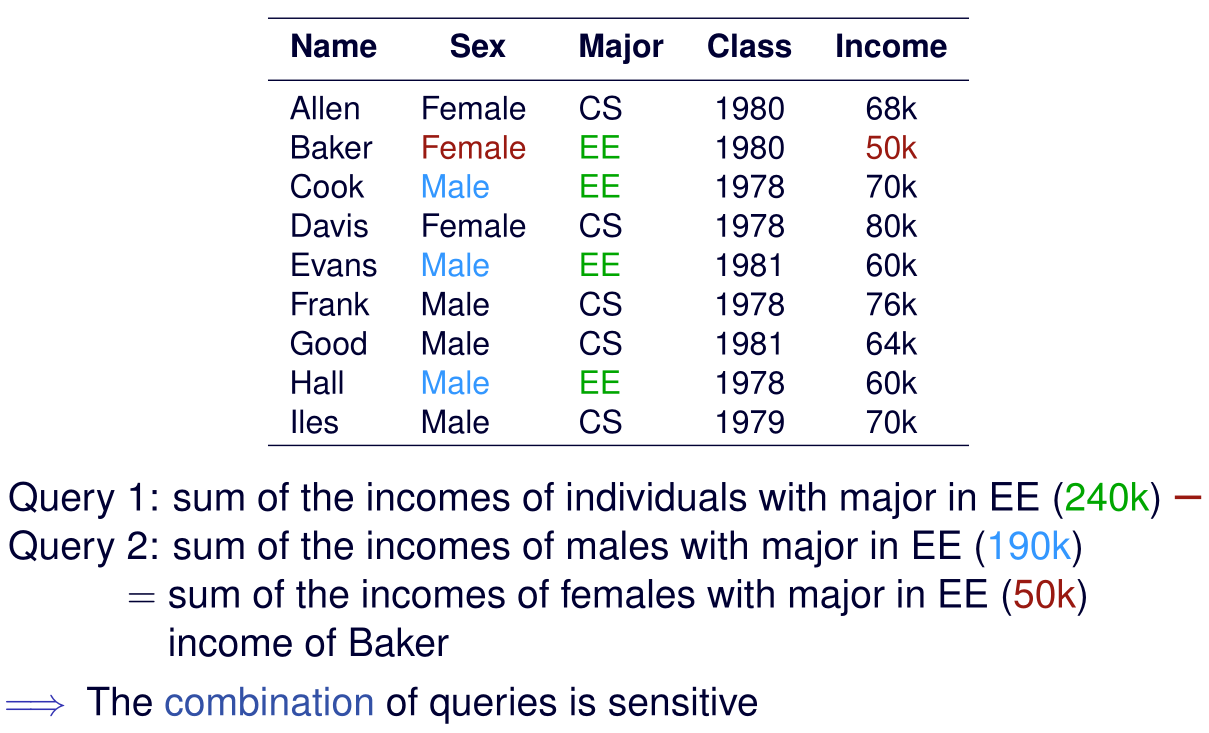
\includegraphics[width=1\linewidth]{images/stat-dbms.png}
\end{figure}

Questa è la ragione per cui mi serve il controllo basato sulla 
storia: devo tenere traccia di quello che mi chiedi e della 
conoscenza che hai, e quindi di cosa puoi inferire.

\chapter{Protezione dei Macrodati}


































\newpage

\section{Macrodata and Microdata Protection}

\subsection{Statistical DBMS vs Statistical Data}
\noindent \textbf{DBMS statistici} - Interazione interattiva tra Client e DBMS:
\begin{itemize}
    \item Il sistema risponde solo a query statistiche.
    \item Necessario un controllo dinamico per proteggere la privacy e prevenire il rilascio indiretto di informazioni.
\end{itemize}

\noindent \textbf{Dati statistici} - Interazione non interattiva tra Client e DBMS:
\begin{itemize}
    \item Pubblicano statistiche (macrodata release).
    \item Il controllo sul rilascio indiretto viene eseguito prima della pubblicazione.
\end{itemize}

\subsection{Statistical DBMS}
Un \textit{DBMS Statistico} è un sistema di gestione di database che fornisce accesso a statistiche su gruppi di individui. 
Deve garantire che non venga rivelata alcuna informazione su un individuo specifico.

\paragraph{Deduzione di informazioni confidenziali}
Tali informazioni possono essere dedotte in vari modi, tra cui:
\begin{itemize}
    \item combinando i risultati di statistiche differenti
    \item combinando i risultati delle statistiche con conoscenza esterna (anche ev. sul contenuto del DB)
\end{itemize}

\subsection{Sensitive Query}
Una \textit{sensitive query} è una query che può provocare una \textit{disclosure}, ovvero la rivelazione di informazioni sensibili su un individuo (es: income molto elevato identifica un individuo peculiare).
Le query, prese singolarmente, potrebbero non essere sensibili, ovvero non rivelare informazioni confidenziali. 
Tuttavia, un insieme di query considerate nel loro complesso può diventare sensibile. Questo fenomeno è noto come \textit{collusione}. 
Attraverso la collusione, le informazioni aggregate da query non sensibili possono portare alla deduzione di dati privati o confidenziali.

\subsection{Macrodata}
Le \textit{Macrodata Tables} possono essere classificate nei seguenti due gruppi (tipi di tabelle):
\begin{itemize}
    \item \textbf{Count/Frequency:} Ogni cella contiene il numero (conteggio) o la percentuale (frequenza) di rispondenti che hanno lo stesso valore su tutti gli attributi nella tabella.
    \item \textbf{Magnitude Data:} Ogni cella contiene un valore aggregato di una quantità di interesse (somma, media, \dots) su tutti gli attributi nella tabella.
\end{itemize}

\section{Macrodata Disclosure Prot. Techniques: Tables of C or F}

\subsection{Data Protection in Count/Frequency Tables}
I dati raccolti dalla maggior parte dei sondaggi sono pubblicati in tabelle di conteggio o frequenze.\\ 
Le tecniche di protezione per tali dati operano in 3 passi:
\begin{enumerate}
    \item \textbf{Sampling}
    \item \textbf{Identification of sensitive cells}
    \begin{itemize}
        \item \textbf{Special Rules}
        \item \textbf{Threshold Rules}
    \end{itemize}
    \item \textbf{Protection of sensitive cells}
    \begin{itemize}
        \item \textbf{Table Restructuring}
        \item \textbf{Suppression}
        \item \textbf{Rounding}
        \item \textbf{Confidentiality Edit}
    \end{itemize}
\end{enumerate}

\subsection{Sampling}
Condurre (e pubblicare) un \textit{sample survey} piuttosto che un censimento.
\begin{itemize}
    \item Le stime vengono effettuate moltiplicando le risposte individuali per un peso di campionamento (\textit{sampling weight}) prima di aggregarle.
    \item Se i pesi non vengono pubblicati, il \textit{weighting} aiuta a rendere i dati di un singolo rispondente meno identificabili dai totali pubblicati.
    \item Le stime devono raggiungere una precisione specificata $\rightarrow$ i dati che non soddisfano i requisiti di precisione non vengono pubblicati (non sono considerati significativi).
\end{itemize}


\subsection{Special Rules}
Quando le \textit{Macrodata Tables} sono definite sull'intera popolazione, necessarie procedure di limitazione della disclosure. 
Le \textit{special rules} definiscono restrizioni sul livello di dettaglio fornito in una tabella.
\begin{itemize}
    \item Le \textit{special rules} variano a seconda del dominio applicativo considerato e del tipo di tabella.
    \item Per soddisfare le \textit{special rules}, si possono applicare:
    \begin{itemize}
        \item \textbf{Table Restructuring}
        \item \textbf{Category Combination}
    \end{itemize}
\end{itemize}

\subsubsection{Esempi di special rules}
Le \textit{special rules} possono richiedere di evitare situazioni in cui un valore in una tabella è uguale a un totale marginale, oppure in cui i dati consentono agli utenti di determinare:

\begin{itemize}
    \item l'età di un individuo all'interno di un intervallo di cinque anni
    \item il reddito all'interno di un intervallo di $1,000$
    \item i benefici all'interno di un intervallo di $50$
\end{itemize}

\subsection{Threshold Rules}
Una cella è considerata sensibile se il numero di rispondenti è inferiore a un certo numero specificato (ad esempio, alcune agenzie considerano 5, altre 3). 
Una cella sensibile non può essere divulgata.
Diverse tecniche possono essere applicate per proteggere le celle sensibili:
\begin{itemize}
    \item \textbf{Table Restructuring \& Category Combination}
    \item \textbf{Cell Suppression}
    \item \textbf{Random Rounding}
    \item \textbf{Controlled Rounding}
    \item \textbf{Confidentiality Edit}
\end{itemize}

\subsection{Table Restructuring}
Per proteggere la riservatezza, la tabella può essere ristrutturata e righe o colonne possono essere combinate (\textit{rolling-up categories}). 2 righe $\rightarrow$ 1 riga aggregata (analogo per colonne).

\subsection{Cell Suppression}
Una delle modalità più comuni per proteggere le celle sensibili è la \textit{suppression}.\\
Rimuovere i valori presenti nelle celle sensibili (\textbf{primary suppression}) non è sufficiente. 
\begin{itemize}
    \item È necessario sopprimere almeno un'altra cella (\textbf{complementary suppression}) per ogni riga o colonna contenente una cella sensibile dalla \textbf{primary suppression}. 
    \begin{itemize}
        \item Altrimenti il valore nella cella sensibile può essere calcolato dal totale marginale.
    \end{itemize}
    \item Anche con la \textbf{complementary suppression}, è difficile garantire una protezione adeguata.
\end{itemize}

\subsection{Complementary Suppressions}
La selezione delle celle per la \textit{complementary suppression} è complicata. 
\begin{itemize}
    \item Vengono utilizzate tecniche di programmazione lineare per selezionare automaticamente le celle da sopprimere. Queste tecniche consentono di formulare il problema di soppressione come un modello matematico, in cui l'obiettivo è massimizzare o minimizzare una funzione obiettivo soggetta a determinati vincoli.
    \begin{itemize}
        \item In questo contesto, la funzione obiettivo potrebbe essere la minimizzazione del numero di celle soppresse o la massimizzazione della protezione dei dati sensibili.
        \item I vincoli possono includere requisiti di riservatezza, come il numero minimo di celle da sopprimere in ogni riga/colonna e la necessità di mantenere la validità statistica dei dati.
    \end{itemize}
    \item Tecniche di audit possono essere applicate per valutare il modello di soppressione proposto e verificare se fornisce la protezione richiesta.
\end{itemize}

\subsection{Rounding}
Per ridurre la perdita di dati dovuta alla soppressione, si utilizza il \textit{rounding} dei valori a un multiplo della soglia di sensibilità.
Esistono due approcci possibili:
\begin{itemize}
    \item \textbf{Random Rounding}: In questa tecnica, si prende una decisione casuale su come arrotondare i valori delle celle, sia verso l'alto (eccesso) che verso il basso (difetto). 
    \begin{itemize}
        \item Il risultato di questo approccio è che la somma dei valori in una riga o colonna potrebbe differire dai totali marginali pubblicati $\rightarrow$ perdita di fiducia nei dati da parte dei destinatari, poiché non possono ricavare con precisione le informazioni aggregate.
    \end{itemize}
    \item \textbf{Controlled Rounding}: Questa tecnica garantisce che la somma delle voci pubblicate sia uguale ai totali marginali pubblicati. 
    \begin{itemize}
        \item Nonostante l'arrotondamento, le informazioni aggregate rimangono coerenti e affidabili.
    \end{itemize}
    \item \textbf{Nota}: Tutti i valori delle celle devono essere un multiplo del valore del \textit{sensitivity threshold}. 
    Fondamentale per mantenere la riservatezza e l'integrità dei dati dopo il \textit{rounding process}.
\end{itemize}

\subsection{Controlled Rounding}
\paragraph{Vantaggi:}
Garantisce che i dati pubblicati siano coerenti con i totali marginali e riduce il rischio di deduzione di informazioni sensibili.

\paragraph{Svantaggi:}
Richiede l'uso di programmi informatici specializzati per l'implementazione e le soluzioni di arrotondamento controllato potrebbero non esistere sempre per tabelle complesse.

\subsection{Confidentiality Edit}
La \textit{Confidentiality Edit} è stata sviluppata dal U.S. Census Bureau per fornire protezione alle tabelle preparate utilizzando il Censimento del 1990. Questa tecnica si basa su due approcci distinti:
\begin{itemize}
    \item \textbf{Protezione dei dati del Censimento decennale regolare} (100\% della popolazione).
    \item \textbf{Protezione Long-Form del Censimento} (campione della popolazione).
\end{itemize}

\noindent Entrambi gli approcci applicano tecniche di \textbf{statistical disclosure limitation} ai microdati sui quali sono calcolate le statistiche, protezione ottenuta mediante la modifica dei dati di input.

\paragraph{Procedura di Switching per il file di microdati al 100\% $\rightarrow$} 
Per il file di microdati al 100\% (1° caso), la \textit{confidentiality edit} si applica attraverso un processo di switching:
\begin{enumerate}
    \item Prendere un campione di record dal file di microdati.
    \item Trovare una corrispondenza per tali record in un'altra regione geografica, effettuando il matching in base a un insieme specifico di attributi importanti.
    \item Scambiare tutti gli attributi sui record corrispondenti.
\end{enumerate}

\noindent Per piccoli blocchi, la frazione di campionamento può essere aumentata per fornire una protezione aggiuntiva. 
Se aumentiamo la frazione di campionamento e decidiamo di includere più soggetti nel campione, ci saranno più dati a disposizione e più variabilità, 
riducendo il rischio di identificare singoli residenti basandosi sui risultati. Inoltre, il file di microdati può essere utilizzato direttamente per preparare tabelle di macrodata, 
mantenendo le correlazioni statistiche ottenibili dai  \textit{raw data}.


\section{Macrodata Disclosure Prot. Techniques: Tables of M}

\subsection{Data Protection in Magnitude Tables}
I \textit{Magnitudine Data} sono generalmente quantità non negative riportate in sondaggi o censimenti. È probabile che la distribuzione di questi valori sia asimmetrica (skewed). Le tecniche di limitazione della divulgazione si concentrano sulla prevenzione della stima precisa dei valori per gli outlier.

\begin{itemize}
    \item Esempi: informazioni su redditi, spese o altre quantità aggregate.
    \item Le tecniche di protezione si concentrano principalmente su come gestire i valori estremi (\textit{outliers}), maggiormente a rischio di disclosure di informazioni sensibili.
    \item Il campionamento è meno efficace nel fornire protezione (NO riservatezza \textit{outliers}).
\end{itemize}

\noindent La protezione delle tabelle di dati di magnitudine implica diversi passaggi fondamentali:
\begin{enumerate}
    \item \textbf{Identification of sensitive cells}
    \begin{itemize}
        \item \textbf{p-percent}: soglia percentuale sotto la quale i valori possono essere considerati sensibili.
        \item \textbf{pq}: combinazione di valori che possono rivelare informazioni riservate.
        \item \textbf{(n,k)}: criterio basato su dimensioni per identificare celle sensibili.
    \end{itemize}
    
    \item \textbf{Protection of sensitive cells}
    \begin{itemize}
        \item \textbf{Suppression}: tecnica comune utilizzata per prevenire la divulgazione di dati riservati.
    \end{itemize}
    
    \item \textbf{Verify result}
    \begin{itemize}
        \item \textbf{Audit}: processo che verifica se le tecniche di protezione sono state applicate correttamente.
        \item \textbf{Information loss}: analisi dell'\textit{information loss} per garantire la significatività dei dati.
        \item \textbf{Parameters are not disclosed}: importante per mantenere la riservatezza dei dati.
    \end{itemize}
\end{enumerate}

\subsection{Suppression Rules - 1}

Le \textit{regole di soppressione} sono fondamentali per proteggere le informazioni sensibili nelle tabelle di dati. Esse si concentrano su due aspetti principali:

\begin{itemize}
    \item \textbf{Regole di Soppressione Primarie}: Determinano se una cella potrebbe rivelare informazioni su un singolo rispondente. Se una cella è considerata sensibile, non può essere rilasciata.
    \item \textbf{Regole di Soppressione Comuni}: Le regole più comuni includono:
    \begin{itemize}
        \item \textit{p-percent rule}: Stabilisce una soglia percentuale al di sotto della quale i valori delle celle sono considerati sensibili.
        \item \textit{pq rule}: Si basa sulla combinazione di variabili per determinare la sensibilità delle celle.
        \item \textit{(n,k) rule}: Utilizza un criterio dimensionale per identificare le celle sensibili.
    \end{itemize}
\end{itemize}

\paragraph{Verifica della Sensibilità}
Queste regole sono utilizzate per identificare celle sensibili verificando se è sufficientemente difficile per un rispondente stimare il valore riportato da un altro rispondente in modo troppo preciso.

\subsection{Suppression Rules - 2}
Le \textbf{Primary Suppression Rules} determinano se una cella potrebbe rivelare informazioni su un singolo rispondente $\rightarrow$ in tal caso tali celle sono considerate sensibili e non possono essere rilasciate.
Le regole di soppressione più comuni sono:
    \begin{itemize}
        \item la \textit{the p-percent rule}
        \item la \textit{the pq rule}
        \item la \textit{the (n,k) rule}
    \end{itemize}
Queste regole vengono utilizzate per identificare celle sensibili verificando se è sufficientemente difficile per un rispondente stimare con accuratezza il valore riportato da un altro rispondente.

\subsection{Primary Suppression Rule: p-percent}
Tale regola stabilisce che la divulgazione di informazioni sensibili a partire dai \textit{Magnitude Data} si verifica se l'utente può stimare troppo accuratamente il contributo di un rispondente. 
\begin{itemize}
    \item Una cella è considerata \textbf{sensibile} se le stime superiori e inferiori per il valore del rispondente sono più vicine al valore riportato di una percentuale predefinita \( p \).
    \item Formalmente, una cella è considerata protetta se:
    \[
    \sum_{i=c+2}^{N} x_i \geq \frac{p}{100} x_1
    \]
    dove:
    \begin{itemize}
        \item \( x_1, x_2, \ldots, x_N \): valori dei rispondenti in ordine decrescente,
        \item \( c \): dimensione di una coalizione di rispondenti interessati a stimare \( x_1 \) (\textit{collusione}).
        \item il valore più grande \( x_1 \) è il più esposto (\textit{outlier}).
    \end{itemize}
\end{itemize}

\subsection{Primary Suppression Rule: pq}
La \textbf{p-percent rule} assume che non ci sia alcuna conoscenza precedente sui valori dei rispondenti. Tuttavia, le agenzie non dovrebbero fare questa assunzione.
\begin{itemize}
    \item Nella regola pq, le agenzie possono specificare quanto sia nota precedentemente l'informazione assegnando un valore \( q \), che rappresenta quanto accuratamente i rispondenti possono stimare il valore di un altro rispondente prima che i dati vengano pubblicati (\( p < q < 100 \)).
    \item Il parametro \( q \) rappresenta l'errore nell'estimazione prima che la cella venga pubblicata.
    \item Formalmente, una cella è considerata protetta se:
    \[
    \frac{q}{100} \sum_{i=c+2}^{N} x_i \geq \frac{p}{100} x_1
    \]
    dove:
    \begin{itemize}
        \item \( x_1, x_2, \ldots, x_N \): valori dei rispondenti in ordine decrescente,
        \item \( c \): dimensione di una coalizione di rispondenti interessati a stimare \( x_1 \) (\textit{collusione}).
        \item il valore più grande \( x_1 \) è il più esposto (\textit{outlier}).
        \item la \textit{pq rule} si riduce alla \textit{p-percent rule} quando \( q = 100 \) (cioè, nessuna capacità di stima).
    \end{itemize}
\end{itemize}

\subsection{Primary Suppression Rule: (n,k)}
Tale regola stabilisce che, indipendentemente dal numero di rispondenti in una cella, se un numero ridotto (\( n \) o meno) di questi rispondenti contribuisce a una grande percentuale (\( k\% \) o più) del valore totale della cella, la cella è considerata sensibile.

\begin{itemize}
    \item \textbf{Regola Intuitiva}: Se una determinata cella è dominata da un solo rispondente, il totale pubblicato rappresenta una stima superiore per il suo valore.
    \item Il valore \( n \) è selezionato per essere maggiore del numero di eventuali coalizioni sospettate.
    \item Molte agenzie utilizzano una regola \( (n,k) \) con \( n = 1 \) o \( n = 2 \).
\end{itemize}

\noindent Esempio: n = 2 \& k = 70: cella sensibile se 2 tuple contengono f(info sensibile) $>$ 70\% tot \\ (f: sum or avg or \dots)

\subsection{Secondary Suppression}
Una volta identificate le celle sensibili, ci sono due opzioni:
\begin{itemize}
    \item \textbf{Ristrutturare la tabella} e combinare le celle fino a quando non rimangono più celle sensibili.
    \item \textbf{Soppressione delle celle}: non pubblicare celle sensibili (\textit{Primary Suppression}) e rimuovere altre celle (\textit{Secondary Suppression}). 
    Un modo amministrativo per evitare la soppressione delle celle consiste nell'ottenere un permesso scritto dai rispondenti.
\end{itemize}


\begin{itemize}
    \item \textbf{Secondary Sup:} è necessario selezionare altre celle non sensibili per la \textit{suppression} per garantire che i dati a livello di rispondente nelle celle sensibili non possano essere stimati con troppa accuratezza
    $\rightarrow$ i dati di un rispondente non possono essere stimati troppo dettagliatamente.
    \item Le celle sensibili potrebbero essere divulgate a causa del fatto che:
    \begin{itemize}
        \item le unioni delle celle soppresse possono essere sensibili secondo la regola di sensibilità adottata,
        \item le equazioni delle righe e delle colonne rappresentate dalla tabella pubblicata possono essere risolte, e il valore per una cella soppressa stimato con troppa accuratezza.
    \end{itemize}
\end{itemize}

Qualsiasi soppressione complementare è accettabile fintanto che le celle sensibili sono protette:
\begin{itemize}
    \item Per tabelle piccole, la selezione delle celle complementari può essere fatta manualmente.
    Gli analisti dei dati sanno quali celle sono di maggiore interesse e non dovrebbero essere utilizzate per la soppressione complementare. 
    La selezione manuale delle celle complementari è accettabile purché la tabella risultante fornisca una protezione sufficiente per le celle sensibili.
    \item  Un audit automatizzato dovrebbe essere applicato per garantire che ciò sia vero.
\end{itemize}

\subsection{Audit}
Se i totali vengono pubblicati, la somma delle celle soppresse (primary/secondary) può essere derivata. È necessario applicare la regola di sensibilità a queste somme per garantire che non siano sensibili.
\begin{itemize}
    \item Le righe e le colonne possono essere viste come un grande sistema di equazioni lineari.
    \item Stimare un \textit{lower bound} e \textit{upper bound} di ciascuna cella soppressa utilizzando \textit{linear programming}.
    \item Se i limiti sono troppo vicini al valore originale, la cella è considerata sensibile.
\end{itemize}

\noindent Semplice per tabelle piccole, ma potrebbe risultare computazionalmente infattibile per tabelle grandi.

\subsection{Information Loss}
La selezione delle celle complementari dovrebbe comportare una minima perdita di informazioni. 
Non esiste una definizione unica di perdita di informazioni.
\begin{itemize}
    \item Ad esempio, possiamo cercare di minimizzare:
    \begin{itemize}
        \item la somma dei valori soppressi (alto numero di celle con valori piccoli può essere soppresso),
        \item il numero totale di celle soppresse.
    \end{itemize}
\end{itemize}

\subsection{Information in Parameter Values}
Mentre le \textit{sup rules} possono essere pubblicate, i valori dei parametri dovrebbero rimanere riservati. 
Una volta che il valore di una cella soppressa è stato determinato in modo univoco, i valori delle altre celle sono facilmente derivabili.

\section{Microdata}

\subsection{Macrodata vs Microdata}
In passato, i dati venivano principalmente rilasciati in forma tabellare (macrodata) e DBMS. 
Oggi, molte situazioni richiedono che i dati specifici memorizzati, chiamati microdata, siano rilasciati. 

\begin{itemize}
    \item Aumento della flessibilità e disponibilità delle informazioni per i destinatari.
    \item I microdata sono soggetti a un maggiore rischio di violazioni della privacy (linking attacks).
\end{itemize}

\subsection{Microdata}
Per proteggere la privacy dei rispondenti, i data owner spesso rimuovono/crittografano identificatori espliciti come nomi, indirizzi e numeri di telefono. Tuttavia, la de-identificazione dei dati non offre alcuna garanzia di anonimato.
Le informazioni rilasciate spesso contengono altri dati quasi identificativi (ad esempio, razza, data di nascita, sesso e codice postale) che possono essere collegati a informazioni disponibili pubblicamente per reidentificare i rispondenti o ridurre l'incertezza sulle loro identità. 
I destinatari dei dati possono determinare (o limitare l'incertezza) a quale rispondente si riferiscono alcuni dati rilasciati. Questo ha creato una crescente domanda nel dedicare risorse per una protezione adeguata dei dati sensibili.
Le tecniche di protezione dei microdata seguono due strategie principali:
\begin{itemize}
    \item ridurre il contenuto informativo (P),
    \item modificare i dati in modo che il contenuto informativo venga mantenuto il più possibile (NP).
\end{itemize}


\subsection{Microdata Disclosure Protection Techniques}
Per limitare il rischio di divulgazione, devono essere applicate le seguenti procedure:
\begin{itemize}
    \item Inclusione di dati provenienti solo da un campione dell'intera popolazione.
    \item Rimozione degli identificatori.
    \item Limitazione dei dettagli geografici.
    \item Limitazione del numero di variabili.
\end{itemize}

\subsection{Classification of Microdata Protection Techniques}
Queste tecniche si basano sul principio che la reidentificazione può essere contrastata riducendo la quantità di informazioni rilasciate:
\begin{itemize}
    \item Mascheramento dei dati (ad esempio, non rilasciando o perturbando i loro valori).
    \item Rilascio di valori plausibili al posto di quelli reali.
\end{itemize}

\noindent Secondo questo principio, le tecniche di protezione possono essere classificate in due categorie principali:
\begin{itemize}
    \item \textbf{Masking techniques (perturbative or not perturbative)}
    \item \textbf{Synthetic data generation techniques}
\end{itemize}

\subsection{Microdata Types}
Le tecniche di protezione possono operare su diversi tipi di dati:
\begin{itemize}
    \item \textbf{Continuous}. attr. definito continuo se numerico e su di esso sono definite operazioni aritmetiche.
    \textbf{Esempio}: data di nascita, temperatura, ecc.
    
    \item \textbf{Categorical}. attr. definito categorico se può assumere un insieme limitato e specificato di valori e le operazioni aritmetiche non hanno senso su di esso.
    \textbf{Esempio}: stato civile, razza, ecc.
\end{itemize}


\section{Microdata Disclosure Prot. Techniques: Masking}

\subsection{Masking Techniques}
Le tecniche di masking trasformano i dati originali per produrre nuovi dati che sono validi per l'analisi statistica e che preservano la riservatezza dei rispondenti. Esse sono classificate come segue:
\begin{itemize}
    \item \textbf{Non-perturbative}: i dati originali non vengono modificati, ma alcuni dati vengono soppressi e/o alcuni dettagli vengono rimossi.
    \item \textbf{Perturbative}: i dati originali vengono modificati.
\end{itemize}

\subsection{Sampling}
La tabella di microdata protetta è ottenuta come un campione della tabella di microdata originale. 
Incertezza riguardo alla partecipazione di un rispondente $\rightarrow$ il rischio di reidentificazione diminuisce.

\subsection{Local Suppression}
La local suppression sopprime il valore di un attributo (cioè lo sostituisce con un valore mancante), limitando così le possibilità di analisi. 
Questa tecnica annulla alcuni valori degli attributi/celle sensibili che potrebbero contribuire in modo significativo al rischio di divulgazione della tupla coinvolta.

\subsection{Global Recoding}
Il global recoding comporta la suddivisione del dominio di un attributo in diversi intervalli disgiunti, tipicamente della stessa ampiezza, e ad ogni intervallo è associata \textit{label}. 
La tabella di microdata protetta è ottenuta sostituendo i valori dell'attributo con la label associata all'intervallo corrispondente.

\subsection{Top-coding e Bottom-coding}
Il top-coding definisce un limite superiore (top-code) per ciascun attributo da proteggere. Qualsiasi valore maggiore di questo limite viene sostituito con un flag che informa l'utente del top-code e indica che il valore supera questo limite. Questa tecnica può essere applicata ad attributi categorici che possono essere ordinati linearmente, così come ad attributi continui.
Analogo per bottom-coding rispetto al limite inferiore (bottom-code).

\subsection{Generalization}
La generalization sostituisce i valori con valori più generali. È tipicamente basata sulla definizione di una gerarchia di generalizzazione, dove il valore più generale è la radice e le foglie corrispondono ai valori più specifici. 
Possono essere costruite diverse tabelle di microdata generalizzate, a seconda del numero di passi di generalizzazione applicati.

\subsection{Random Noise}
Il random noise perturba un attributo sensibile aggiungendo o moltiplicando il valore di quest'ultimo con una variabile casuale di una distribuzione specificata. 
È necessario decidere se pubblicare o meno la distribuzione/i utilizzata/e per aggiungere rumore ai dati. 
La pubblicazione della distribuzione/i potrebbe aumentare il rischio di divulgazione dei dati (Disclosure di Informazioni Sensibili).

\subsection{Swapping}
Una piccola percentuale di record viene abbinata con altri record nello stesso file, forse in diverse regioni geografiche, su un insieme di variabili predeterminate. 
I valori di tutte le altre variabili nel file vengono quindi scambiati tra i record selezionati. Questa tecnica riduce il rischio di reidentificazione poiché introduce incertezza riguardo al valore reale dei dati di un rispondente.

\subsection{Micro-aggregation (Blurring)}
La micro-aggregation consiste nel raggruppare tuple individuali in piccoli gruppi di dimensione fissa \( k \). Viene pubblicata la media di ciascun gruppo invece dei valori individuali. I gruppi sono formati utilizzando criteri di massima similarità. Ci sono diverse variazioni della micro-aggregazione:
\begin{itemize}
    \item la media può sostituire il valore originale solo per una tupla nel gruppo o per tutte;
    \item diversi attributi possono essere protetti attraverso la micro-aggregazione utilizzando lo stesso o diversi raggruppamenti;
    \item \ldots
\end{itemize}


\section{Microdata Disclosure Prot. Techniques: Synthetic}

\subsection{Synthetic techniques}
Poiché il contenuto statistico dei dati non è correlato alle informazioni fornite da ciascun rispondente, un modello che rappresenti bene i dati potrebbe, in linea di principio, sostituire i dati stessi. 
Un requisito importante per la generazione di dati sintetici è che tali dati e quelli originali devono presentare la stessa qualità nell'analisi statistica. Il principale vantaggio di questa classe di tecniche è che i dati sintetici rilasciati non sono riferiti a nessun rispondente e, pertanto, il loro rilascio non può portare a reidentificazione.







\end{document}